\chapter{Transfer Function}
\label{chap:tf}
The transfer function was calculated from the system equation
\eqref{eq:equationmotion} analysed in the section
\ref{subsec:equationofomotion}, where the input is \(g_{\text{v}}\).
To calculate the transfer function between the force and the positions, the 
voltage-to-force coefficient gain has to be removed.
%
\begin{equation}
\label{eq:gs}
	G(s) = \big([M]s^2+[C]s+[K]\big)^{-1}
\end{equation}
%
Given \(F(s)\) we obtain the Laplace transform of the force signal.
The transfer function is a column vector with three entries, one for each output,
they share the denominator as in eq.\eqref{eq:gs}.
%
\begin{equation}
\label{eq:tf}
	\frac{X(s)}{F(s)} = \frac{1}{g_{\text{v}}}\,\frac{X(s)}{V(s)}
\end{equation}
%
\begin{figure}[htb]
	\centering
	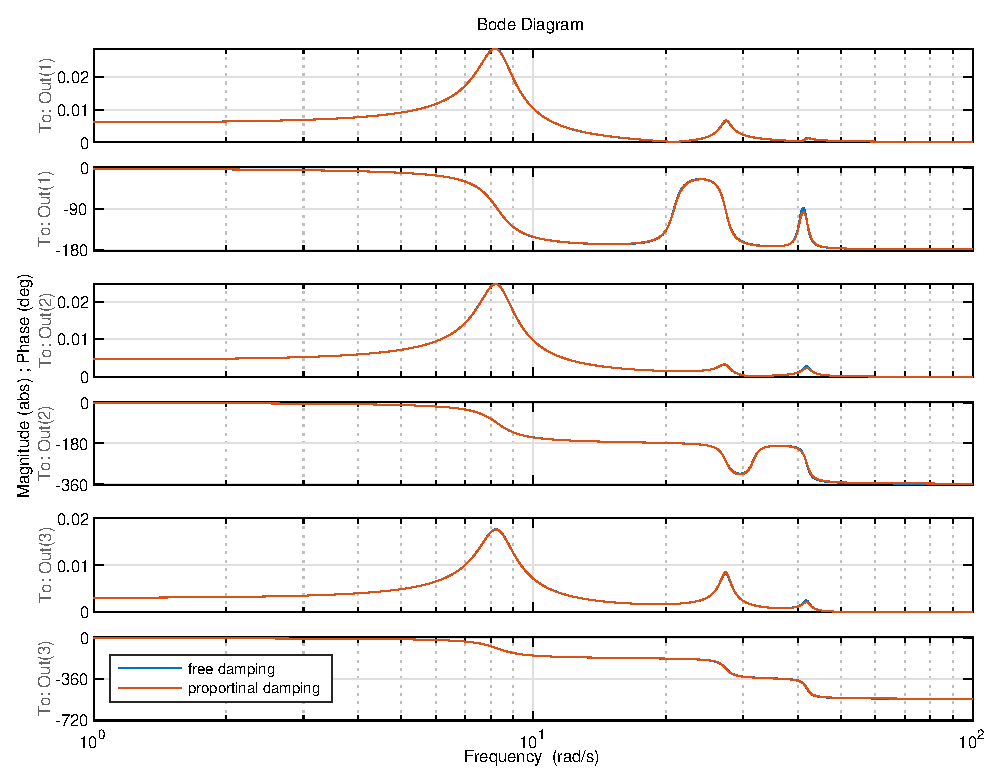
\includegraphics[width=0.64\textwidth]{bodediagram1}
	\caption{Bode diagram of the transfer functions as in \eqref{eq:tf}}
	\label{fig:bodeplot1}
\end{figure}
%
The bode diagram are shown in Figure \ref{fig:bodeplot1}.